\documentclass[spanish,a4paper,10pt]{article}

\usepackage{latexsym,amsfonts,amssymb,amstext,amsthm,float,amsmath}
\usepackage[spanish]{babel}
\usepackage[utf8]{inputenc}
\usepackage[dvips]{epsfig}
\usepackage{doc}
\usepackage[T1]{fontenc}
\usepackage[dvips]{graphicx}

\begin{document}
\title{Aproximación del número $\pi$}
\author{Rebeka Luis Hernández}
\date{11 de abril de 2014}

\maketitle

\begin{abstract}
El objetivo de esta práctica es entregar un programa escrito en \textsf{Latex}
en el que se aproxime el valor de $\pi$ con un una precisión dada.
\end{abstract}
%++++ Aqui comenzamos con la primera sección+++

\section{Historia del número pi}

A lo largo de la historia han sido muchas las formas utilizadas por el ser humanos para calcular aproximaciones 
cada vez más exactas del número $\pi$. El número $\pi$ es el cociente entre la longitud de una circunferencia 
cualquiera y el diámetro de la misma. Ludolph van Ceulen (1540-1610), matemático alemán profesor de la 
Universidad de Leiden en Holanda, se pasó buena parte de su vida calculandolos primeros 35 decimales de $\pi$.

%++Aqui comenzamos con la segunda sección+++

\section{Cálculo del número pi}

Calcularemos una aproximación del número $\pi$ mediante la siguiente \footnote fórmula{Aunque también s epuede calcular mediante integración} :

\begin{center}
$ \pi \approx \frac{1}{n} \sum\limits_{i=1}^{n}f(x_i)\,$,
con $f(x) = \frac{4}{(1+x^2)}\,$,
$x_i = \frac{i - \frac{1}{2}}{n}$,
para $i = , \dots, n$
\end{center}

Además realizaremos una serie de pasos que enumeraremos a continuación:

%+++ Enumeramos las subsecciones
\begin{enumerate}
  \item
    Calculo de los extremos de los subintervalos.
  \item
    Calculo del punto $x_i$.
  \item
    El valor de la función de aproximación de $pi$, $f(x_i)$.
\end{enumerate}
Para ver más detallado el proceso observaremos el siguiente gráfico:
\begin{figure}{h}
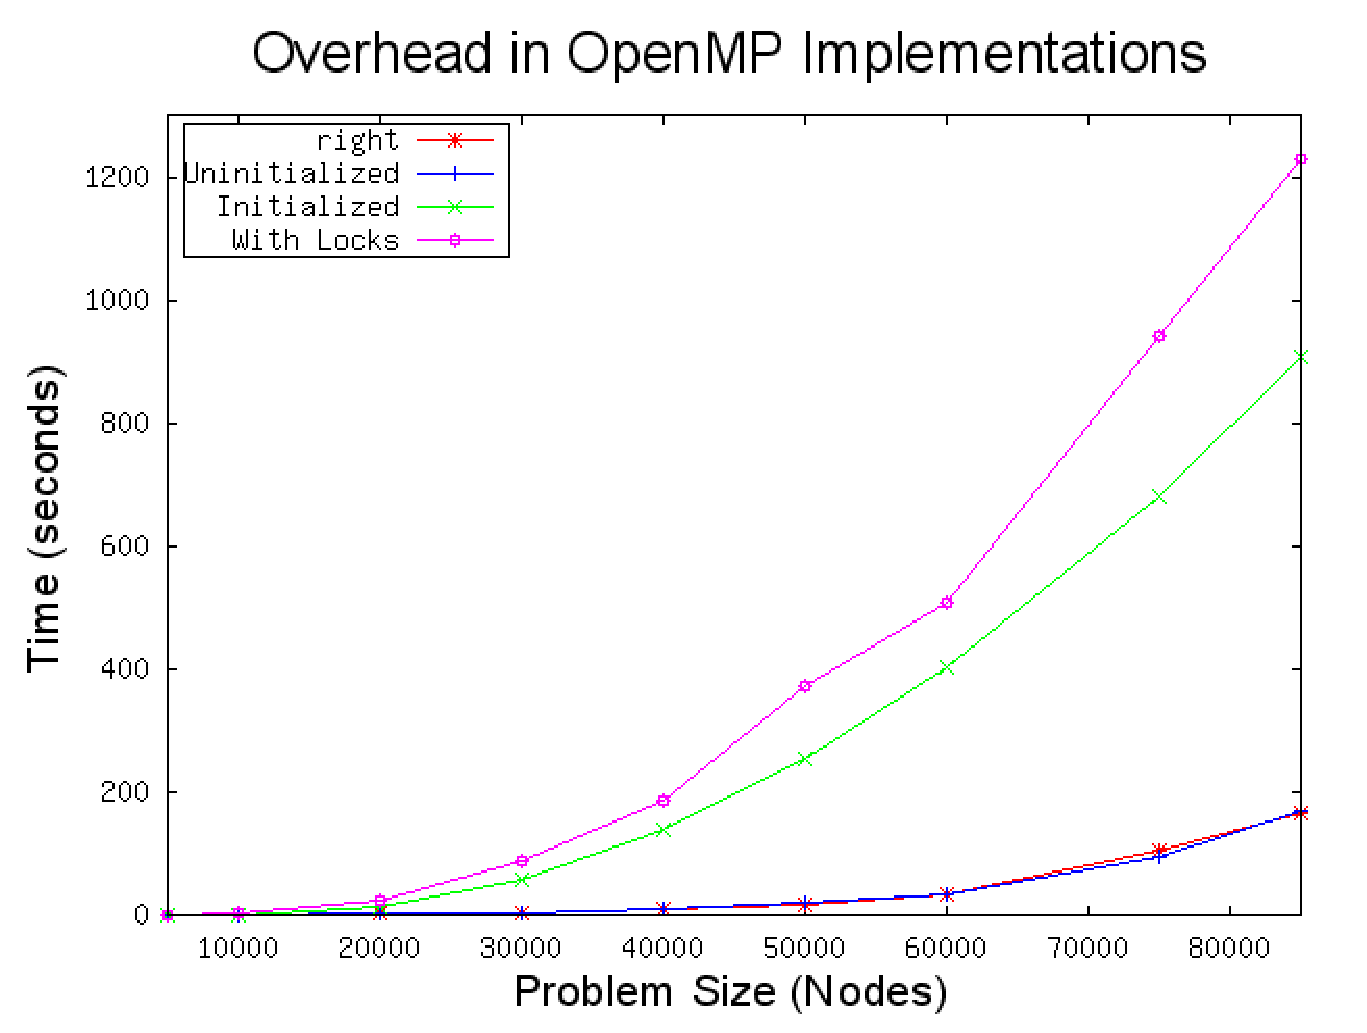
\includegraphics[scale=1]{figura.eps}
\caption{Figura 1}
\label{contexto:figura}
\end{figure}
 


\section{Ejemplo}

Por ejemplo, si utiliza 3 \footnote subintervalos{El valor de la n debe ser mayor que cero}, la salida debería ser:


\begin{table}{!h}
\label{Mitabla}
\begin{tabular}{rcc}

Subintervalo: [0 ,0.25] & $x_i$: 0.125  & $fx_i$: 3.93846 \\
Subintervalo: [0.25, 0.5] & $x_i$: 0.375  & $fx_i$: 3.50685 \\
Subintervalo: [0.5, 0.75] & $x_i$: 0.625  & $fx_i$: 2.8764 \\

\end{tabular}
\end{table}

Para observar ejemplo ir a \ref{Mitabla}.

\begin{thebibliography}{2}
\bibitem{python} Tutorial de Python. http://docs.python.org/2/tutorial/
\bibitem{latex} Tutorial de Latex.  http://campusvirtual.ull.es/1314/course/view.php?id=1447
\end{thebibliography}


\end{document}






